\documentclass{beamer}
\usetheme{default}
\usepackage{amsmath}
\usepackage{amsfonts}
\usepackage{amssymb}
\usepackage{booktabs}
\usepackage{graphicx}
\usepackage{enumerate}
\usepackage{xeCJK}
\usepackage{zhnumber}
\usepackage{listings}
\usepackage{float}
\setCJKmainfont[BoldFont=FZHei-B01]{FZShuSong-Z01}
\setCJKfamilyfont{hei}{FZHei-B01}
\setCJKfamilyfont{kai}{FZKai-Z03}
\setCJKfamilyfont{fang}{FZFangSong-Z02}
\newcommand{\hei}{\CJKfamily{hei}}
\newcommand{\kai}{\CJKfamily{kai}}
\newcommand{\fang}{\CJKfamily{fang}}

\usepackage{fontspec}
\newfontfamily\mymono{Source Code Pro}
\usepackage{color}
\definecolor{mygreen}{rgb}{0,0.6,0}
\definecolor{mygray}{rgb}{0.5,0.5,0.5}
\definecolor{mymauve}{rgb}{0.58,0,0.82}
\lstset{
	%frame=single,
	numbers=left,
	numberstyle=\footnotesize\mymono\color{mygray},
	basicstyle=\footnotesize\mymono,
	breaklines=true,
	tabsize=4,
	commentstyle=\color{mygreen},
	keywordstyle=\color{blue},
	stringstyle=\color{mymauve},
	showstringspaces=false
}

\title{OpenMP\\\ \\
	An Easy Way for Parallel Programming
	}
\author{Chuizheng Meng}
\date{\today}

\begin{document}
	\begin{frame}
		\titlepage
	\end{frame}
	
	\section{What is OpenMP}
	\begin{frame}
		\frametitle{\insertsection}
		\begin{itemize}
			\item OpenMP is a specification for a set of compiler directives, library routines, and environment variables that can be used to specify high-level parallelism in Fortran and C/C++ programs.
			\item OpenMP is designed for Fortran, C and C++.
			\item Supported compilers
			\begin{itemize}
				\item GCC($\geqslant$ 4.2.0)
				\item Visual Studio 2008-2010 C++
				\item Clang($\geqslant$ 3.8)
				\item IBM, Intel, Texas Instrument...
			\end{itemize}
			\item Only a supported compiler is needed!
		\end{itemize}
	\end{frame}
	
	\section{Hello OpenMP}
	\begin{frame}[fragile]
		\frametitle{\insertsection}
		\begin{block}{hello.cpp}
		\begin{lstlisting}[language=C++]
#include <stdio.h>

int main() {
    #pragma omp parallel
    printf("Hello OpenMP!\n");
    return 0;
}\end{lstlisting}
		\end{block}
		\begin{block}{Compile\ \&\ Run(with flag "-fopenmp")}
		\begin{lstlisting}[language=bash]
g++ -Wall -Werror -O3 hello.cpp -o hello -fopenmp
./hello\end{lstlisting}
		\end{block}
\end{frame}
	\begin{frame}
		\frametitle{\insertsection}
		\begin{block}{Result}
			\begin{figure}[H]
				\centering
				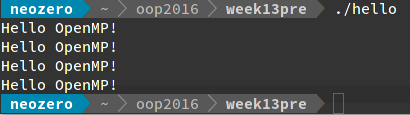
\includegraphics[width=\linewidth]{helloopenmp.png}
			\end{figure}
		\end{block}
	\end{frame}
	
	\section{How OpenMP Works}
	\begin{frame}
		\frametitle{\insertsection}
		\begin{block}{Fork-Join Model}
		\begin{figure}[H]
			\centering
			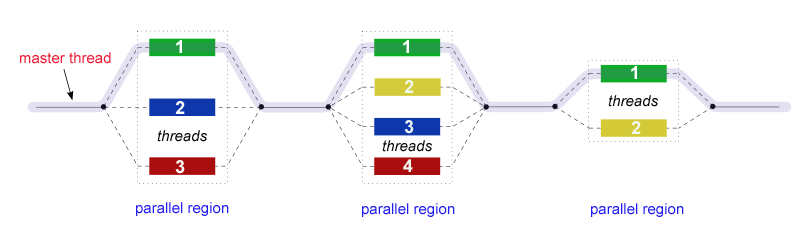
\includegraphics[width=\linewidth]{fork_join2.png}
		\end{figure}
		\end{block}
		\begin{itemize}
			\item All OpenMP programs begin as a single process: the master thread.
			\item Fork
			\item Join
		\end{itemize}
	\end{frame}
	\begin{frame}
		\frametitle{\insertsection}
		\begin{itemize}
			\item Shared Memory Model
			\item Thread Based Parallelism
			\item Explicit Parallelism
			\item Compiler Directive Based
			\item Dynamic Threads
			\item I/O(It is your duty!)
		\end{itemize}
	\end{frame}
	
	\section{OpenMP API Overview}
	\begin{frame}
		\frametitle{\insertsection}
		\begin{itemize}
			\item Compiler Directives
			\item Runtime Library Routines
			\item Environment Variables
		\end{itemize}
	\end{frame}
	
	\section{Compiler Directives}
	\begin{frame}[fragile]
		\frametitle{\insertsection}
		\begin{block}{Format}
		\begin{lstlisting}[language=C++,numbers=none]
#pragma omp directive-name [clause,...]\end{lstlisting}\end{block}
\end{frame}
	\subsection{Directive-name}
	\begin{frame}
		\frametitle{\insertsubsection}
		\begin{itemize}
			\item parallel
				\begin{itemize}
					\item A parallel region is a block of code that will be executed by multiple threads.
					\item It is the fundamental OpenMP parallel construct.
				\end{itemize}
			\item for
				\begin{itemize}
					\item Shares iterations of a loop across the team.
					\item Data parallelism
				\end{itemize}
			\item sections
				\begin{itemize}
					\item Each section is executed by a thread.
					\item Functional parallelism
				\end{itemize}
			\item single
				\begin{itemize}
					\item The enclosed code is to be executed by only one thread in the team. Other threads will never execute it.
					\item Can be used to deal with IO.
				\end{itemize}
		\end{itemize}
	\end{frame}
	\begin{frame}
		\frametitle{\insertsubsection}
		\begin{itemize}
			\item critical
			\begin{itemize}
				\item Only ONE thread can execute codes in the block at same time.
				\item Often used when a shared variable is modified.
			\end{itemize}
			\item atomic
			\begin{itemize}
				\item A unit of storage can only be modified by ONE thread at same time.
				\item Often used when some value of a shared array is modified.
			\end{itemize}
		\end{itemize}
	\end{frame}
	
	\subsection{Clause}
	\begin{frame}
		\frametitle{\insertsubsection}
		\begin{figure}[H]
			\centering
			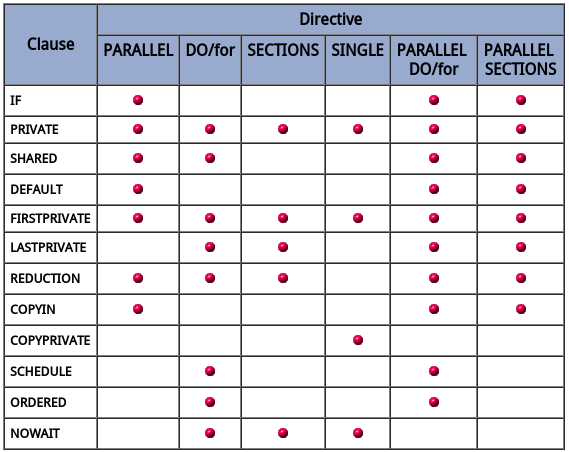
\includegraphics[width=0.8\linewidth]{clause.png}
		\end{figure}
	\end{frame}
	\begin{frame}
		\frametitle{\insertsubsection}
		\begin{itemize}
			\item if (expression)\begin{itemize}
				\item True: A team of threads is created.
				\item False: The region is executed serially by the master thread.
			\end{itemize}
			\item private(list) \begin{itemize}
				\item Variables in the list is private to each thread.
				\item They should be assumed to be uninitialized for each thread.(Use firstprivate to solve that.)
			\end{itemize}
			\item shared(list) \begin{itemize}
				\item Variables in the list is shared among all threads.
				\item It is the programmer's responsibility to ensure that multiple threads properly access shared variables!
			\end{itemize}
		\end{itemize}
	\end{frame}
	\begin{frame}
		\frametitle{\insertsubsection}
		\begin{itemize}
			\item reduction(op:list) \begin{itemize}
				\item Performs a reduction on the variables that appear in its list.
				\item Operator must observe commutative law and associative law.
				\item For some variable x in list, multiple private copies of x is created in each thread, and finally x is set as (x op x op x op ... op x).
			\end{itemize}
			\item schedule(kind[, chunksize]) \begin{itemize}
				\item Automatically arrange "working schedule" for different threads of for loop.
				\item Chunksize: size of each piece of work.
				\item Kind: method to distribute work, including static, dynamic, guided and runtime.
			\end{itemize}
		\end{itemize}
	\end{frame}
	\begin{frame}
		\frametitle{\insertsubsection}
		\begin{itemize}
			\item schedule(kind[, chunksize])
			\begin{itemize}
				\item Kind
				\begin{itemize}
					\item static: loop
					\item dynamic: first come, first serve
					\item guided: like dynamic, but with descending chunksize
					\item runtime: follow the env value OMP\_SCHEDULE
				\end{itemize}
			\end{itemize}
		\end{itemize}
		\begin{figure}[H]
			\centering
			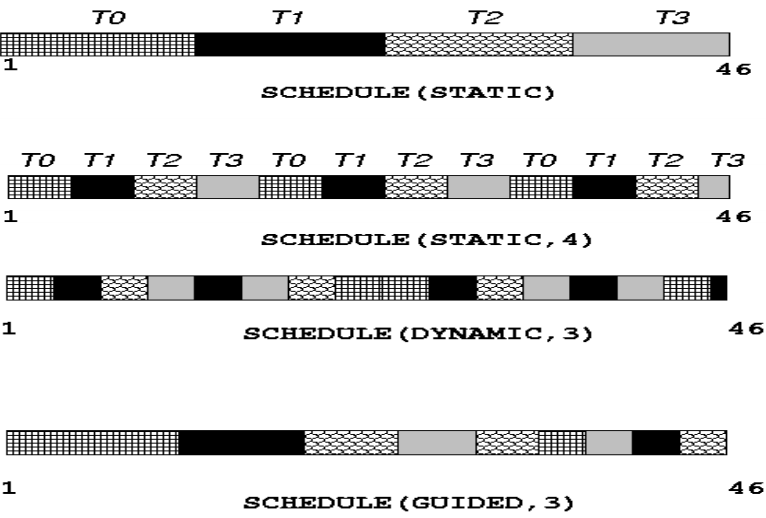
\includegraphics[width=0.8\linewidth]{schedule.png}
		\end{figure}
	\end{frame}
	\begin{frame}
		\frametitle{\insertsubsection}
		\begin{block}{Static}
			\begin{figure}[H]
				\centering
				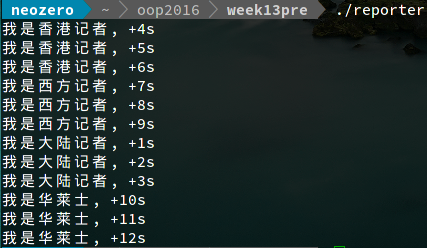
\includegraphics[width=0.8\linewidth]{sche_static.png}
			\end{figure}
		\end{block}
	\end{frame}
	\begin{frame}
		\frametitle{\insertsubsection}
		\begin{block}{Dynamic}
			\begin{figure}[H]
				\centering
				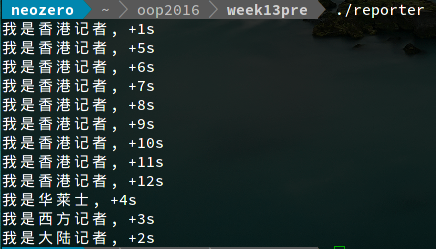
\includegraphics[width=0.8\linewidth]{sche_dynamic.png}
			\end{figure}
		\end{block}
	\end{frame}
	\begin{frame}
		\frametitle{\insertsubsection}
		\begin{block}{Guided}
			\begin{figure}[H]
				\centering
				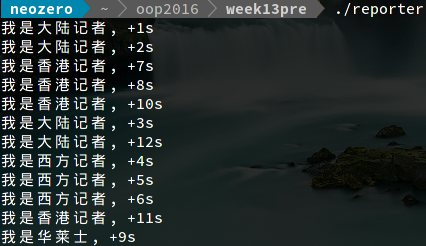
\includegraphics[width=0.8\linewidth]{sche_guided.png}
			\end{figure}
		\end{block}
	\end{frame}
	
	\section{Runtime Library Routines}
	\begin{frame}
		\frametitle{\insertsection}
		\begin{itemize}
			\item For C/C++, include the <omp.h> header file.
			\item void omp\_set\_num\_threads(int num\_threads)
			\item int omp\_get\_num\_threads(void)
			\item int omp\_get\_thread\_num(void)
			\item Manipulations about lock(using critical may be easier)
			\item ...
		\end{itemize}
	\end{frame}
	
	\section{Environment Variables}
	\begin{frame}
		\frametitle{\insertsection}
		\begin{itemize}
			\item OpenMP provides some environment variables for controlling the execution of parallel code.
			\item OMP\_SCHEDULE
			\item OMP\_NUM\_THREADS
			\item OMP\_THREAD\_LIMIT
		\end{itemize}
	\end{frame}
	
	\section{Examples}
	\begin{frame}
		\frametitle{\insertsection}
		\begin{itemize}
			\item Merge Sort with OpenMP
			\item Numeric calculation of $\pi$
		\end{itemize}
	\end{frame}
	\subsection{Merge Sort}
	\begin{frame}[fragile]
		\frametitle{\insertsubsection}
		\begin{lstlisting}[language=C++,numbers=none]
void mergesort(int* array, int start, int end, int thread, int* buffer) {
    if (end - start <= 1)
        return;
    int p = ((start + end) >> 1);
    if (thread <= 1) {
        mergesort(array, start, p, 1, buffer);
        mergesort(array, p, end, 1, buffer);
    }\end{lstlisting}
\end{frame}
	\begin{frame}[fragile]
		\frametitle{\insertsubsection}
		\begin{lstlisting}[language=C++,numbers=none]
    else {
        #pragma omp parallel sections
        {
        #pragma omp section
        {
        mergesort(array, start, p, thread / 2, buffer);
        }
        #pragma omp section
        {
        mergesort(array, p, end, thread - thread / 2, buffer);
        }
        }
    }
    merge(array, start, p, end, buffer);
}\end{lstlisting}
\end{frame}

\begin{frame}
	\frametitle{\insertsubsection}
	\begin{figure}[H]
		\centering
		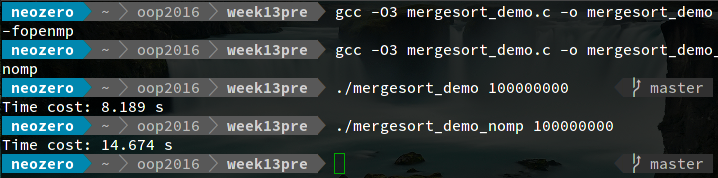
\includegraphics[width=\linewidth]{mergesort.png}
		\end{figure}
\end{frame}

	\subsection{Numeric calculation of $\pi$}
	\begin{frame}
		\frametitle{\insertsubsection}
		\begin{equation}
			\int_{0}^1\dfrac{4}{1+x^2}=4\arctan1=\pi
		\end{equation}
		\begin{equation}
			\int_{0}^1\dfrac{4}{1+x^2}=\lim_{N\rightarrow +\infty}\dfrac{1}{N}\sum_{i=0}^{N-1}\dfrac{4}{1+\left(\frac{i}{N}\right)^2}
		\end{equation}
	\end{frame}
	\begin{frame}[fragile]
		\frametitle{\insertsubsection}
		\begin{lstlisting}[language=C++,numbers=none]
#pragma omp parallel for schedule(static) reduction(+:sum)
for (i = 0; i < MAXSTEP; ++i) {
    sum = sum + FUNC((double)i/MAXSTEP);
}\end{lstlisting}
\begin{figure}[H]
	\centering
	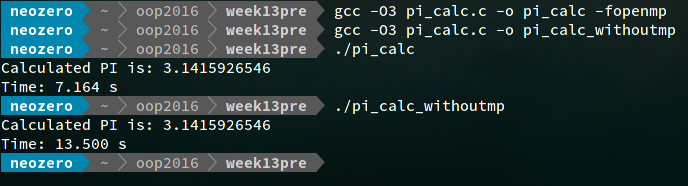
\includegraphics[width=\linewidth]{pi.png}
\end{figure}
\end{frame}

	\section{Pros\ \&\ Cons}
	\begin{frame}
		\frametitle{\insertsection}
		\begin{itemize}
			\item Pros \begin{itemize}
				\item Make full use of CPU with little work.
				\item Portable multithreading code, not platform-specific.
				\item Work can be easily scheduled.
				\item Unified code for both serial and parallel applications.
			\end{itemize}
			\item Cons \begin{itemize}
				\item High chance of accidentally writing false sharing code.
				\item Difficult to debug.
				\item Not very suitable for some situation, i.e. network programming.
				\item Mainly for parallel computing, not for distributed computing.
			\end{itemize}
		\end{itemize}
	\end{frame}

	\section{Reference}
	\begin{frame}
		\frametitle{\insertsection}
		\begin{itemize}
			\item \footnotesize "OpenMP" - Blaise Barney, Lawrence Livermore National Laboratory\\https://computing.llnl.gov/tutorials/openMP/
			\item \footnotesize OpenMP并行编程 - 中国科学技术大学超级计算中心\\http://scc.ustc.edu.cn/zlsc/cxyy/200910/W020121113517997951933.pdf
			\item \footnotesize OpenMP - Wikipedia\\
			https://en.wikipedia.org/wiki/OpenMP
		\end{itemize}
	\end{frame}

\end{document}